\renewcommand{\topfraction}{1.0}
\setcounter{topnumber}{100}

As described in the previous section, a test method is being developed that
will be suitable for comparing the performance of different kitting
planning systems. The method looks at plans that are an ordered sequence
of actions for a robot to perform. The actions are specified in terms of
the canonical robot command language (CRCL).

\subsubsection{Kitting Viewer Introduction}
A software tool named the ``kittingViewer'' is being developed that will
read files describing the initial state, the goal state, and the plan for
getting from the initial state to the goal state. The kittingViewer will
simulate execution of the plan, display a view of the plan being executed,
and produce and display metrics about the plan.  All of the metrics will be
numbers. All but one of the metrics will be objective and require no human
judgement. The final metric will be a subjective combination of the other
metrics in which the other metrics will be weighted and combined as desired
by the user.

The kittingViewer is partially built. It is able to read in the three
input files and simulate execution of the plan file. Plan metrics are
being calculated, and robot motion is being animated at speeds specified
in the plan.

A sample plan file is shown in Figure~\ref{fig:KittingPlan}. The file is
designed for exercising the kittingViewer and is not intended to make sense
as a plan. It includes a few intentional errors.

Figure~\ref{fig:KittingViewer} shows the kittingViewer display at its
current state of development. The display uses three windows, labelled
Metrics \& Settings, Kitting Viewer, and Kitting Command. The windows may
be moved and resized independently, like other windows in a typical
windowing system. The image in the Kitting Viewer window resizes when the
window is resized, but the text in the other two windows does not
change size when the windows change size, so there is little point in
resizing them.

The Kitting Viewer window shows a view of the kitting workstation. The
floor of the workstation is covered with a grid. The spacing of the grid is
the last entry in the Metrics and Settings window. The robot in the
workstation is represented by a gantry robot spanning the entire width of
the workstation.  The gantry robot moves when any of the CRCL motion
commands is executed.  The speed at which the picture of the robot is
animated matches the actual commanded speed of the robot.  When development
of the kittingViewer is complete, objects in the workstation will also be
shown (in color) and will move if the robot moves them.

The Kitting Command window shows the currently executing command or the
most recently executed command, if no command is currently executing.

\begin{figure*}[ht]
\begin{center}
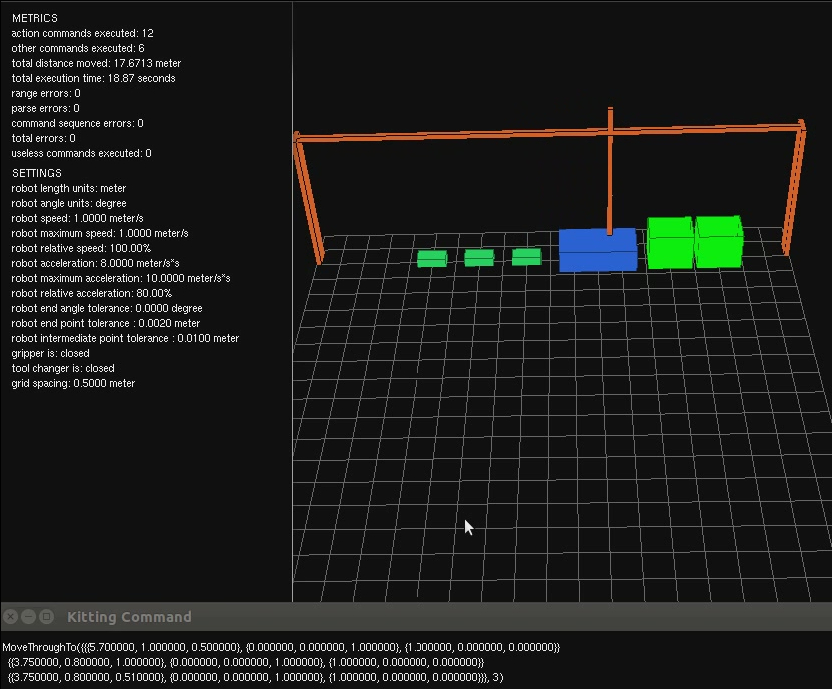
\includegraphics[width=16cm]{images/kittingViewer.jpg}
\caption{Kitting Viewer Display}
\label{fig:KittingViewer}
\end{center}
\end{figure*}

\subsubsection{Kitting Viewer Metrics}
The Metrics \& Settings window shows 9 metrics at the top and 14 settings
below that. All but three of the settings correspond to items that may be
set using CRCL commands. The extra three are the grid spacing and the robot
maximum speed and maximum acceleration (which may not be reset). As
commands are executed, metrics and settings are updated in the window.
When the kittingViewer is completed, there will be more metrics.
Currently, the metrics are:\\

\begin{itemize}

\item \sf action commands executed \rm -- the number of action commands that
  have been executed so far. An action command is any command that takes
  time to execute, namely: Dwell, MoveStraightTo, MoveThroughTo, MoveTo,
  OpenGripper, CloseGripper, OpenToolChanger, and CloseToolChanger.\\

\item \sf other commands executed \rm -- the number of commands that are
  not action commands and have been executed so far -- mostly setting
  commands. Executing these commands is assumed to take a negligible amount
  of time.\\

\item \sf total distance moved \rm -- the total distance covered so
  far. This is calculated as the total of the distances between points in
  the move commands, taken in order (and starting at the place where the
  controlled point is located initially). The value is updated as each point
  is reached, not continuously.\\

\item \sf total execution time \rm -- the total time taken so far by
  executing action commands. This does not include any time that may elapse
  between when one command finishes execution and when the user tells the
  kittingViewer to execute another command. The total execution time is
  meant to be very close to the actual amount of time that would be taken
  by a real robot.\\

\item \sf range errors \rm -- the number of times a command tries to set a
  value that is out of the allowed range of the value. If a range error
  occurs, an error message is printed in the terminal window from which the
  kittingViewer was started. The \sf SetRelativeAcceleration(-110) \rm
  command in Figure~\ref{fig:KittingPlan} causes two range errors, one
  because it is negative, and one because its absolute value is greater
  than 100.\\

\item \sf parse errors \rm -- the number of lines in the CRCL command file
  that cause an error in the command file parser. When the parser
  encounters a line that it cannot parse, it adds an UnreadableMsg to the
  list of commands it has parsed. The UnreadableMsg includes the text of
  the line on which the parse error occurred. When the UnreadableMsg is
  executed, the value of parse errors is increased by one and the
  UnreadableMsg is displayed in the Kitting Command window so the user can
  see the line that caused the problem. The \sf MoveStraightTo(87) \rm
  command in Figure~\ref{fig:KittingPlan} causes a parse error.\\

\item \sf command sequence errors \rm -- the number of commands that are
  out of sequence. An InitCanon command is out of sequence if it is not the
  first command in the file. An EndCanon command is out of sequence if it
  is not the last command in the file. Other commands are out of sequence
  if they occur before InitCanon or after EndCanon.\\

\item \sf total errors \rm -- the sum of the range errors, parse errors,
  and command sequence errors.\\

\item \sf useless command executed \rm -- the number of commands that do
  not change the state of the workstation. Such commands have no effect, so
  they are useless. The \sf CloseGripper() \rm and \sf CloseToolChanger()
  \rm commands in Figure~\ref{fig:KittingPlan} are useless because the
  gripper and tool changer are closed in the initial conditions.\\

\end{itemize}

\subsubsection{Controlling Kitting Viewer}
Controlling the kittingViewer is accomplished by using the mouse and single
keys on the keyboard. When the kittingViewer starts up, a set of one-line
instructions is printed in the terminal window from which the
kittingViewer was started. Those instructions have the same meaning as
the longer explanations given below.\\

\begin{itemize}

\item R key -- The R key toggles the behavior of the left mouse button
  between translating and rotating the picture. This functionality is
  included because some mice do not have a middle button. Press R once and
  the left mouse button controls rotation. Press R again and the the left
  mouse button controls translation (the original setting).\\

\item Left mouse button -- By default, the left mouse button is used to
  translate the picture. Position the cursor anywhere in the Kitting Viewer
  window, hold down the left mouse button and move the cursor by moving the
  mouse. The picture will move as though it is glued to the cursor. If the
  R key has switched the left mouse button to rotation, it behaves like the
  middle mouse button, as described in the next paragraph.\\

\item Middle mouse button -- The middle mouse button is used to rotate the
  picture. This is a little trickier than the other two mouse buttons. To
  rotate the picture, position the cursor inside the window near an edge of
  the window, hold down the middle mouse button, and move the cursor in a
  straight line towards the opposite edge. The picture rotates around an axis
  that is perpendicular to the line of mouse motion. Experiment. In order
  to allow for fine positioning, the amount of rotation that occurs for a
  given amount of mouse motion decreases as the picture is zoomed
  in. Hence, if you want to turn the picture completely over, it is best to
  zoom out, rotate, and zoom back in again.\\

\item Right mouse button -- The right mouse button is used to zoom in or
  out. To zoom out, position the cursor near the bottom of the picture,
  hold down the right mouse button and push the mouse away from you (moving
  the cursor up); that appears to push the picture away from you. To zoom
  in, position the cursor near the top of the picture, hold down the right
  mouse button and pull the mouse toward you (moving the cursor down); that
  appears to pull the picture toward you. Moving the mouse side to side
  while holding down the right mouse button does nothing. There are limits
  to how far in or out you can zoom. At the highest magnification, it is
  easy to see a separation of half a millimeter. This is zooming, not
  moving the point of view, so the eye never goes through the picture.\\

\item H key -- If the h key is pressed, the view in the Kitting Viewer
  window returns to its original position.\\

\item G key -- If the g key is pressed when the plan is not completely
  executed and no action command is executing, the next command in the plan
  is executed and the Metrics \& Settings window is updated. If the g key
  is pressed when the plan is completely executed or when an action command
  is in progress, nothing happens.\\

\item T key -- If the t key is pressed, a combined image of all the windows
  will be saved in a file. The name of the file will be anaglyph\_N.ppm,
  where N starts at 0000 and increases by 1 each time the t key is
  pressed. The ppm (portable pixmap) format is a common graphics format
  that many graphics utilities can handle.\\

\item Z or Q key -- If the z or q key is pressed, the kittingViewer program
  exits, and the windows disappear.\\

\end{itemize}

\subsubsection{Kitting Viewer Development Plans}

As mentioned earlier, the kittingViewer is far from complete. It is
planned to add the following capabilities.

\begin{itemize}

\item Add drawing the kitting workstation in its current state. The initial
  state of the workstation is already available in data as soon as the XML
  data file that describes it is read in. 

\item Add updating the positions of objects as the robot executes commands.
  It will be necessary to compare the position of the robot with the
  positions of objects when OpenGripper and CloseGripper commands are
  executed in order to determine if the robot is grasping them.

\item Add metrics related to the positions of objects. This might include
  (1) the number of objects that should have been moved, (2) the number of
  objects that were moved (3) the number of objects that were moved to the
  correct place, (4) the number of objects that were moved to the wrong
  place.

\item Add metrics related to constraint violations. This might include (1)
  the number of instances of picking up an object that weighs more than the
  robot's load capacity, (2) the number of instances of the robot moving
  outside of its work volume, (3) the number of instances of using a
  gripper to move an object when the gripper is not qualified to move the
  object. It will also be necessary to decide what the simulation should do
  in these cases and implement that.

\item Add a total score metric, and implement finding the total score using
  a configuration file in which the user assigns weights to the other
  metrics.

\end{itemize}